% !TeX spellcheck = ru_RU
\chapter{Аналитическая часть}

В данном разделе будут рассмотрены алгоритмы сортировки --- пузырьком, пирамидальная, блочная.

\section{Сортировка пузырьком}
\textbf{Сортировка пузырьком} (BubbleSort) \cite{bubble_source} --- алгоритм сортировки, состоящий из повторяющихся проходов по сортируемому массиву.
За каждый проход элементы последовательно сравниваются попарно и, если порядок в паре неверный, выполняется обмен элементов.
Проходы по массиву повторяются $N-1$ раз, однако существует модифицированная версия, в которой проходы прекращаются, если окажется, что дальнейшая сортировка не нужна (массив уже отсортирован).
При каждом проходе алгоритма по внутреннему циклу очередной наибольший элемент массива ставится на свое место в конце массива рядом с предыдущим наибольшим элементом, а наименьший элемент массива перемещается на одну позицию к началу массива.

\section{Пирамидальная сортировка}
\textbf{Пирамидальная сортировка }(HeapSort) \cite{heapsort_source} --- это метод сортировки сравнением, основанный на такой структуре данных как двоичная пирамида (heap).

\textbf{Двоичная (бинарная) пирамида} --- структура данных, представляющая собой объект-массив, который можно рассматривать как почти полное бинарное дерево, как показано на рис. \ref{fig:heap_exmp}.
\begin{figure}[h]
	\centering
	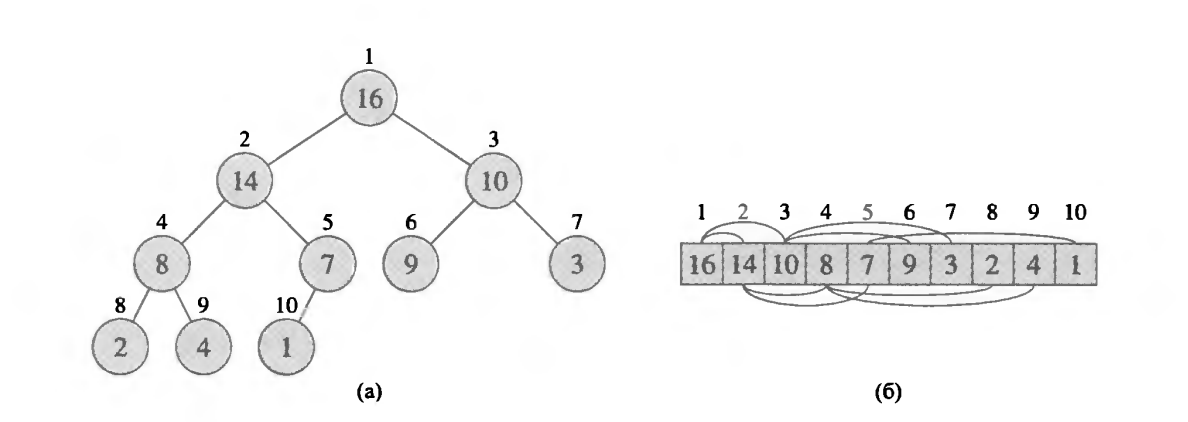
\includegraphics[width=\linewidth]{img/heap_example.png}
	\caption{Невозрастающая пирамида представлена в виде \textbf{(а)} бинарного дерева и в виде \textbf{(б)} массива}
	\label{fig:heap_exmp}
\end{figure}
Каждый узел дерева соответствует элементу массива, дерево полностью заполнено на всех уровнях, за исключением, возможно, низшего, который заполняется слева направо. 
\pagebreak

Различают два вида бинарных пирамид: неубывающие и невозрастающие. 

Для неубывающей пирамиды (max-heap) выполняется свойство \newline $A[Parent(i)] \geqslant A[i]]$о, т.е. значение узла не превышает значения родительского по отношению к нему узла. Таким образом, наибольший элемент пирамиды находится в корне.  

Принцип организации неубывающей пирамиды (min-heap) прямо противоположный и подчиняется закону $A[Parent(i)] \leqslant A[i]$. Таким образом, наименьший элемент такой пирамиды находится в корне.

Поскольку двоичная пирамида — это почти законченное двоичное дерево, ее можно легко представить в виде массива, а представление на основе массива является эффективным с точки зрения расхода памяти. Если родительский узел хранится в индексе $i$, левый дочерний элемент может быть вычислен как $2i + 1$, а правый дочерний элемент — как $2i + 2$.

Алгоритм пирамидальной сортировки сводится к следующим шагам:
\begin{enumerate}
	\item построение невозрастающей пирамиды из входного массива;
	\item обмен максимального значения элемента дерева (в невозрастающей пирамиде находится в корне) и значения элемента с индексом m, где m --- количество элементов дерева;
	\item построение на основе оставшихся элементов двоичной пирамиды размера $m - 1$;
	\item повторение пунктов 2, 3 для полученной под-пирамиды длины $m-1$, пока длина под-пирамиды не станет равна 0.
\end{enumerate} 

В результате работы в области памяти, выделенной для хранения двоичного дерева в начале алгоритма, окажется отсортированный массив, поданный на вход.

Для построения невозрастающей пирамиды из входного массива пользуются процедурой heapify алгоритм которой, описан ниже.

Т.к. двоичное дерево хранится в виде массива, элементы этого массива с индексами [(n/2 + 1)...n] (где n - длина входного массива) представляют собой листья дерева, поэтому каждый из них можно считать тривиальной (одно-элементной) невозрастающей пирамидой. При прохождении узлов с индексами [(n/4 + 1)...n/2], являющихся родительскими по отношению к листьям дерева, считаем, что оба его дочерних элемента являются корнями невозрастающих под-пирамид. 

Процедура heapify для узла с индексом $i \in [0...n/2]$ определяет наибольший из элементов A[i], A[Left(i)], A[Right(i)], где A - массив с числами, Left(i) и Right(i) - левый и правый дочерний элемент соответственно, индекс наибольшего элемента записывается в переменную largest. Если наибольший из трех элементов не является значением элемента A[i], элементы A[i] и A[largest] меняются значениями. Это приводи к тому, что для узла i и его дочерних элементов выполняется свойство невозрастающей пирамиды. Однако теперь исходное значение A[i] оказывается в узле с индексом largest, так что поддерево с корнем largest может нарушать свойство невозрастающей пирамиды. Следовательно, необходимо рекурсивно вызвать процедуру heapify уже для этого дерева.

\section{Блочная сортировка}
\textbf{Блочная сортировка} (Bucket sort) \cite{bucket_source} --- алгоритм сортировки, предполагающий, что входные данные подчиняются равномерному закону распределения; время работы в среднем случае при этом оказывается равным O(n). 

Данный алгоритм сортировки разбивает интервал [a, b] (где a и b - минимальный и максимальный элемент массива соответственно) на n одинаковых интервалов, или \textbf{блоков}(buckets), а затем распределяет по этим блокам n входных чисел. Поскольку последние (согласно предположению) равномерно распределены в интервале [a, b], мы предполагаем, что в каждый из блоков попадет не очень много элементов. Чтобы получить выходную последовательность, нужно просто выполнить сортировку чисел в каждом блоке, а затем последовательно перечислить элементы каждого блока.

В классическом варианте алгоритма каждый блок сортируется при помощи сортировки вставками, однако возможно использование любого другого алгоритма сортировки. В данной лабораторной работе будет рассмотрена реализация алгоритма, использующая сортировку вставками.

\section*{Вывод}
В данном разделе были рассмотрены алгоритмы сортировки --- пузырьком, пирамидальная, блочная.